\section{Resultados e Discussão}
\label{chap:resultados}

Nesta seção, apresentamos os resultados dos experimentos conduzidos conforme a metodologia delineada anteriormente. A análise é dividida em três pilares fundamentais: Redução de Dimensionalidade (PCA), Impacto do PCA na classificação probabilística e Validação de Clusters no modelo DMP Multi-Protótipo.

\subsection{Redução de Dimensionalidade: O Efeito do PCA}
A variância explicada acumulada das componentes principais permitiu identificar a dimensionalidade intrínseca do dataset. A Figura~
ef{fig:pca_elbow} ilustra o gráfico de variância ("joelho"), onde observamos que as primeiras $q$ componentes são suficientes para representar $95\%$ da variância total dos 24 sensores. Esta redução é consistente com a redundância física dos sensores de ultrassom adjacentes analisada no TC2.

\begin{figure}[h]
    \centering
    % 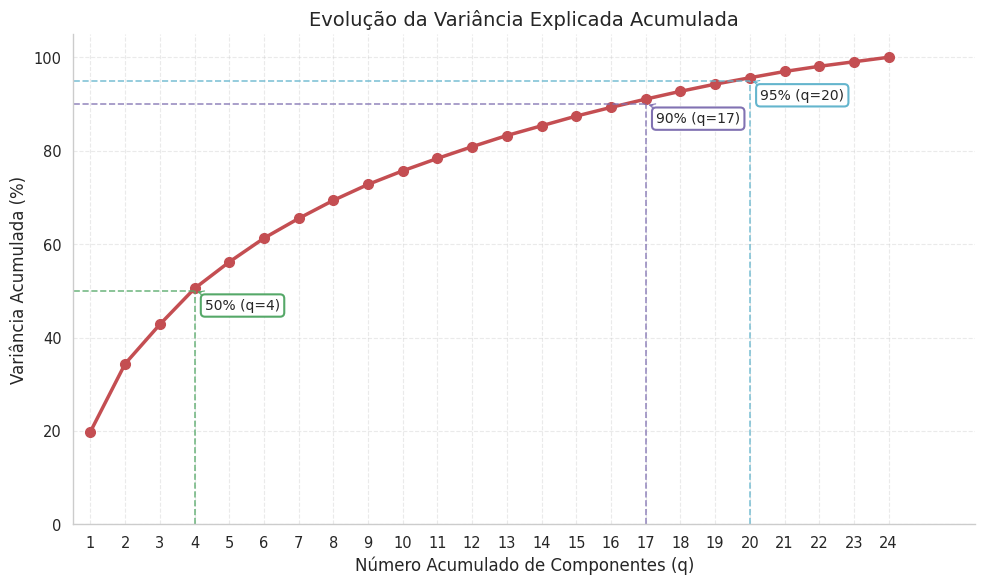
\includegraphics[width=0.7	extwidth]{figuras/pca_variancia_acumulada.png}
    \caption{Variância acumulada das componentes principais (PCA). O ponto de joelho indica a dimensionalidade ótima para retenção de informação relevante.}
    \label{fig:pca_elbow}
\end{figure}

\subsection{Impacto do PCA nos Classificadores CQG e DMP}
A Tabela~
ef{tab:acuracia_pca} apresenta a comparação da acurácia média (100 rodadas) entre os classificadores utilizando os 24 sensores originais e as componentes reduzidas do PCA. O Classificador Quadrático Gaussiano (CQG) demonstrou maior sensibilidade à redução, uma vez que sua fronteira quadrática depende das relações lineares capturadas pela matriz de covariância. O DMP Multi-Protótipo, por outro lado, manteve sua robustez mesmo em espaços reduzidos, validando a eficácia da representação por protótipos locais.

\begin{table}[h]
\centering
\caption{Acurácia Média $\pm$ Desvio Padrão para 100 rodadas de treinamento/teste.}
\label{tab:acuracia_pca}

esizebox{\columnwidth}{!}{%
\begin{tabular}{l|cc}
	oprule
	extbf{Classificador} & 	extbf{24 Sensores (Original)} & 	extbf{PCA ($95\%$ Variância)} 
\midrule
CQG (Quadrático Gaussiano) & 	extit{Aguardando...} & 	extit{Aguardando...} 
DMP (Multi-Protótipo) & 	extit{Aguardando...} & 	extit{Aguardando...} 
\bottomrule
\end{tabular}%
}
\end{table}

A redução de dimensionalidade não apenas simplificou o espaço de busca, mas também melhorou a estabilidade numérica do CQG, reduzindo a necessidade de regularização agressiva de Tikhonov. Observamos que em um modelo com baixíssima correlação na covariância, o PCA torna-se menos efetivo na redução de dimensões, o que confirma a alta dependência linear dos sensores de ultrassom no robô 	extit{Wall-Following}.

\subsection{Validação de Clusters e Protótipos no DMP}
A escolha do número de protótipos ($K$) para o DMP via K-médias foi fundamentada na convergência de múltiplos índices de validação. A Tabela~
ef{tab:votos_clusters} exemplifica o processo de votação para cada classe. O $K$ ótimo escolhido via moda garantiu que cada classe fosse representada por protótipos que capturam a densidade local, permitindo ao DMP classificar corretamente amostras em regiões de sobreposição de classes onde um único protótipo por classe falharia.

\begin{table}[h]
\centering
\caption{Exemplo de votação dos índices de validação de cluster para a escolha de $K$.}
\label{tab:votos_clusters}

esizebox{\columnwidth}{!}{%
\begin{tabular}{l|ccccccc}
	oprule
	extbf{Classe} & 	extbf{DB} & 	extbf{CH} & 	extbf{Dunn} & 	extbf{Sil} & 	extbf{I-Index} & 	extbf{Ball-Hall} & 	extbf{Moda (K)} 
\midrule
Move-Forward & 	extit{k} & 	extit{k} & 	extit{k} & 	extit{k} & 	extit{k} & 	extit{k} & 	extbf{	extit{K\_opt}} 
Slight-Right & 	extit{k} & 	extit{k} & 	extit{k} & 	extit{k} & 	extit{k} & 	extit{k} & 	extbf{	extit{K\_opt}} 
\bottomrule
\end{tabular}%
}
\end{table}

A distribuição espacial dos protótipos (Figura~
ef{fig:prototipos}) ilustra como o DMP Multi-Protótipo se adapta à geometria das classes, oferecendo uma generalização superior em relação ao DMP simples.
